%-------------------------------------------------------------------------------
\section{\sys Overview}
\label{s:overview}
%-------------------------------------------------------------------------------

%
\sys is a library that web application code calls into to invoke data disguises.
%
Web application developers rely on data disguises to help conveniently and
correctly implement application-specific privacy transformations.
%
In particular, \sys guarantees that if a data disguise has disguised an original
application data object $o$ into a disguised object $d$, the original, undisguised
object $o$ is hidden from an attacker who compromises the server as long as it is
not explicitly revealed by its original owner.
%

%
In addition to the privacy-increasing, ``forward'' transformations that disguise
data---\eg account deletion, anonymization, or data decay---\sys also makes it easy for
developers to implement reversal of disguises (``backward'' transformations, \eg when a
user reactivates their account) and operations over disguised data (\eg edits to
anonymized information) while disguised data remains secure.
%

%
Importantly, a application developer who uses \sys needs not to worry about the
cryptographic details or interaction between disguises.
%
Instead, the developer works with a set of abstractions that fit a wide
variety of application use cases.
%

\subsection{Threat Model}
\label{s:threat}

%
Data disguises protect a web application's disguised user data against a
powerful attacker who compromises the web application server and gains full
access to it.
%
As a result of the compromise, the attacker can:
\begin{enumerate}[nosep]
 \item see any information that a user of the web application can access through
   the application;
  \item access all data stored in the web application's database;
  \item access all memory and disk contents, including \sys's data structures; and
  \item perform any operation that the application can perform, including invoking
    \sys API calls.
\end{enumerate}
%
A data disguise guarantees that the disguised data, and any metadata about who applied
which disguise, is hidden from the attacker unless explicitly revealed by the user
for whom it was disguised.
%
Users who are inactive can therefore rest assured that their disguised data, and
its existence, is never exposed.
%
However, while \sys hides who disguised a piece of application data, it does not hide
the existence of disguised data, nor does it protect against informationed leaked from
undisguised data that remains in the application database (\eg a message quoted
within another message).
%

%
Under \sys's threat model, an attacker who compromises \sys at time $t$ therefore
learns \emph{nothing but}:
%
\begin{enumerate}[nosep]
  \item the (plaintext) contents of the application database at or after time $t$;
  \item the total number of disguises invoked and the (rough) amount of data
    disguised by each disguise;
  \item the disguises invoked, and the identity of the users invoking them,
    \emph{after} time $t$; and
  \item any data disguised prior to $t$, if accessed and undisguised by the user
    for whom the data was originally disguised.
\end{enumerate}
%
We make standard assumptions about the security of cryptographic primitives: attackers
cannot break encryption and keys stored with non-colluding clients are safe.
%
\sys operates in an honest-but-curious setting: even if compromised, \sys faithfully
executes its protocols, but their execution leak the data accessed post-compromise.
%


\subsection{Application Developer Perspective}
%
It's the application developer's job to invoke \sys, and \sys is normally
hidden from end users of the web application.
%
However, the web application's UI may expose functionality that invokes \sys's
data disguises behind the scenes, such as a ``Delete my account'' button.
%

%
An application developer devises the privacy transformations their application needs to
support, implements them in terms of \sys's API, and exposes hooks to invoke disguises to
users who are empowered to trigger them (\eg individual users for account deletion, but
administrators for global anonymization).
%

\subsection{\sys Operation}

\begin{figure}[t]
  \centering
    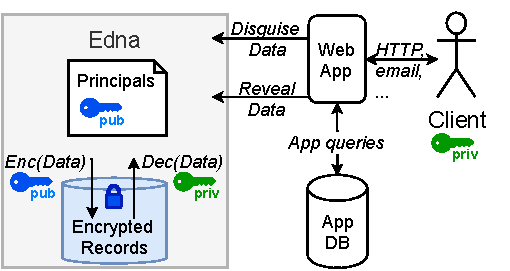
\includegraphics[width=0.5\textwidth]{figs/edna_arch}
  \caption{\sys handles application requests to disguise or reveal data. Only the
    encryption of \sys's stored records is trusted.}
  \label{f:edna-overview}
\end{figure}
